% first frame:
% REAL ROBOTS! REAL-WORLD PROBLEMS!
% overview of manipulation planning problem?
\begin{frame}
   \frametitle{Autonomous Manipulation Tasks}
   \begin{tikzpicture}
      \draw[step=1,black!15,very thin,opacity=\gridopacity] (0,0) grid (12,8);
   
      \node[inner sep=0] at ( 2,5.0) {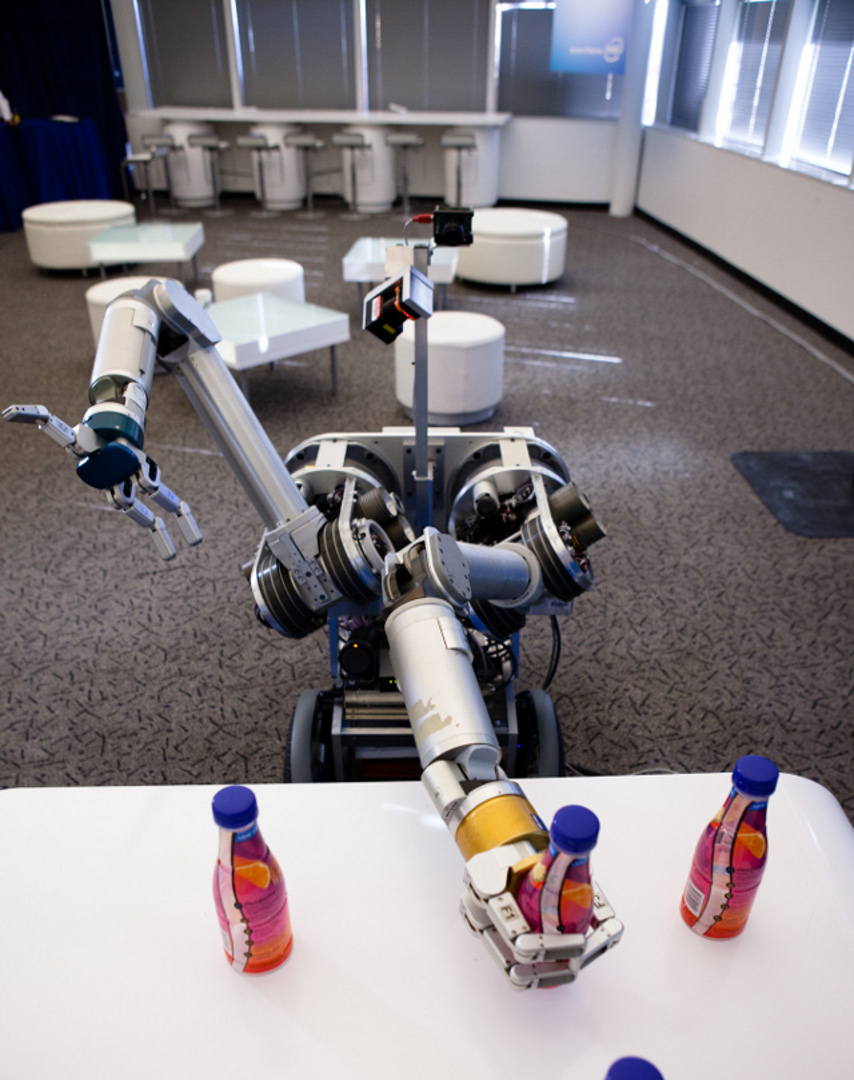
\includegraphics[width=3.5cm]{images/herb.jpg}};
      \node[inner sep=0] at ( 6,5.0) {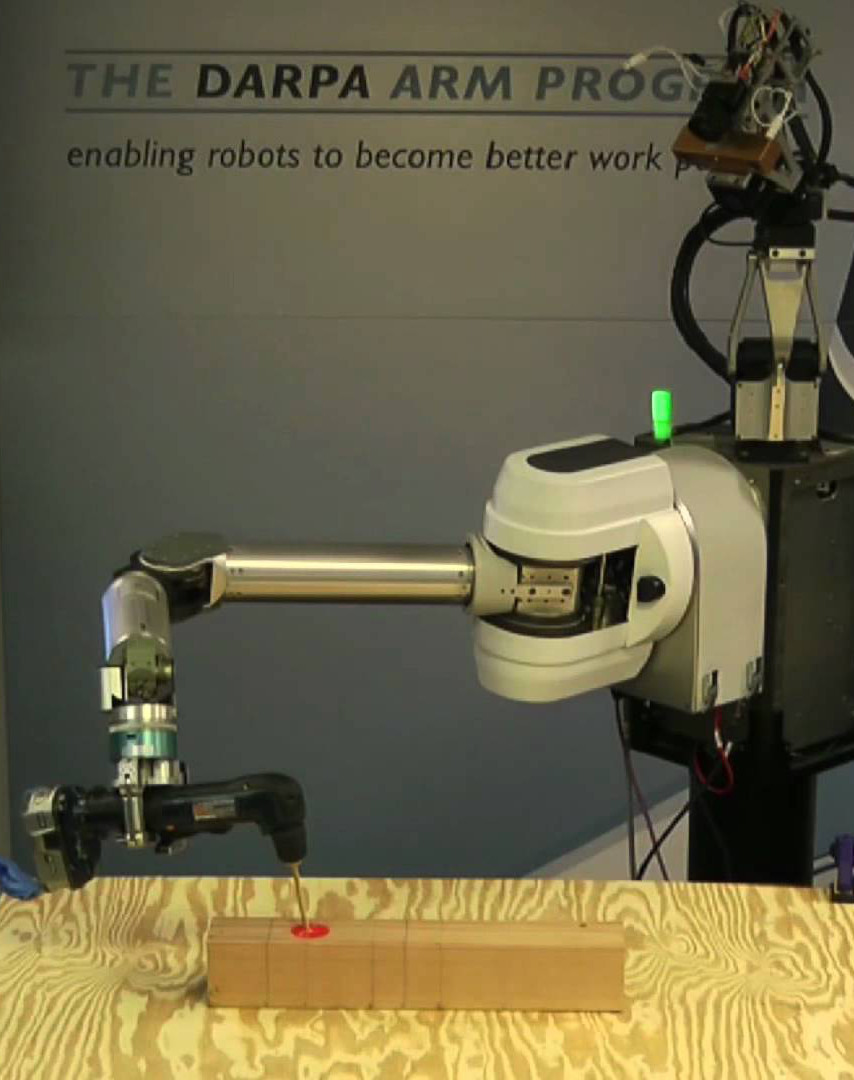
\includegraphics[width=3.5cm]{images/arms.jpg}};
      \node[inner sep=0] at (10,5.0) {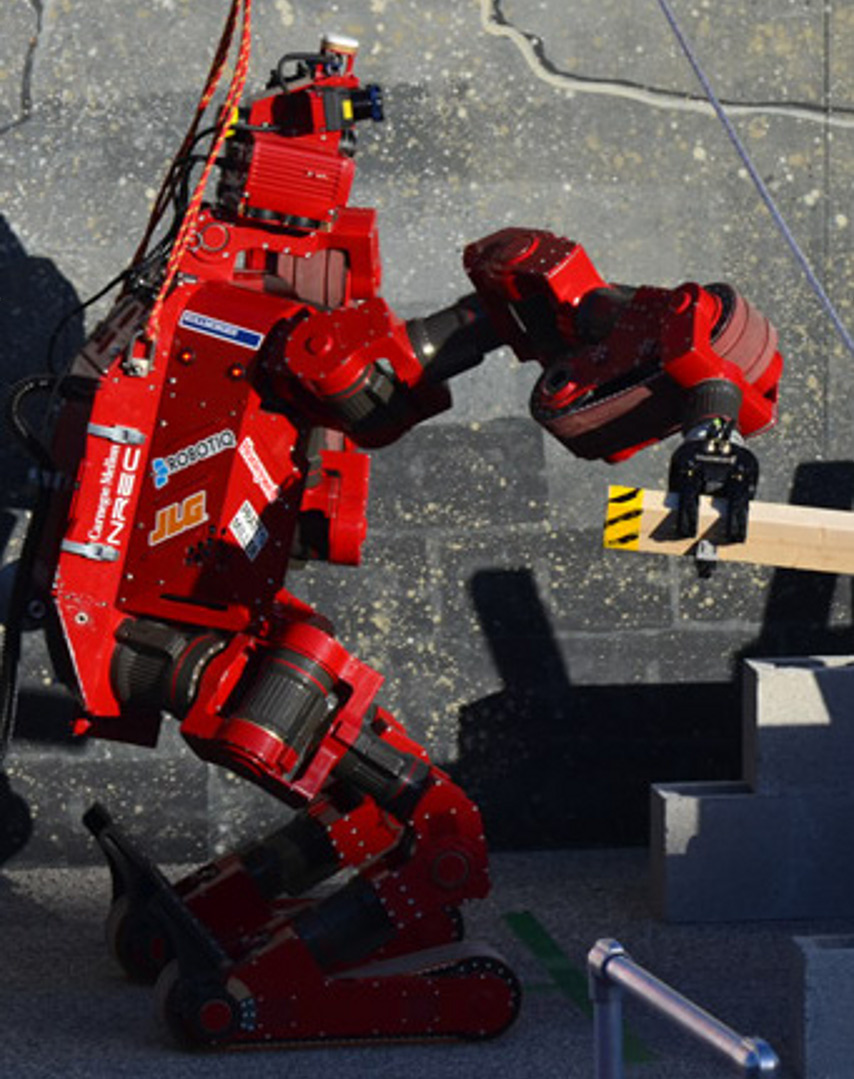
\includegraphics[width=3.5cm]{images/chimp.jpg}};
      \node at ( 2,2.4) {HERB};
      \node at ( 6,2.4) {ARM-S};
      \node at (10,2.4) {CHIMP};
      
      \only<2->{
      \node[fill=blue!20,rounded corners,align=center,minimum height=1.5cm,align=center]
         (sense) at (2,0.85) {Sense\\(build geometric\\world model)};
      }

      \only<3->{
      \node[fill=blue!20,rounded corners,align=center,minimum height=1.5cm,align=center]
         (plan) at (6,0.85) {Plan\\(motion plans)};
      \draw[->,line width=1pt] (sense) -- (plan);
      }

      \only<4->{
      \node[fill=blue!20,rounded corners,align=center,minimum height=1.5cm,align=center]
         (act) at (10,0.85) {Act\\(execute\\motion plans)};
      \draw[->,line width=1pt] (plan) -- (act);
      }
   
   \end{tikzpicture}
\end{frame}

\begin{frame}
   \frametitle{An Example Manipulation Task}
   \begin{tikzpicture}[font=\small]
      \draw[step=1,black!15,very thin,opacity=\gridopacity] (0,0) grid (12,8);

   \node[inner sep=0pt] at (6,5.3) {%
      \only<1-2>{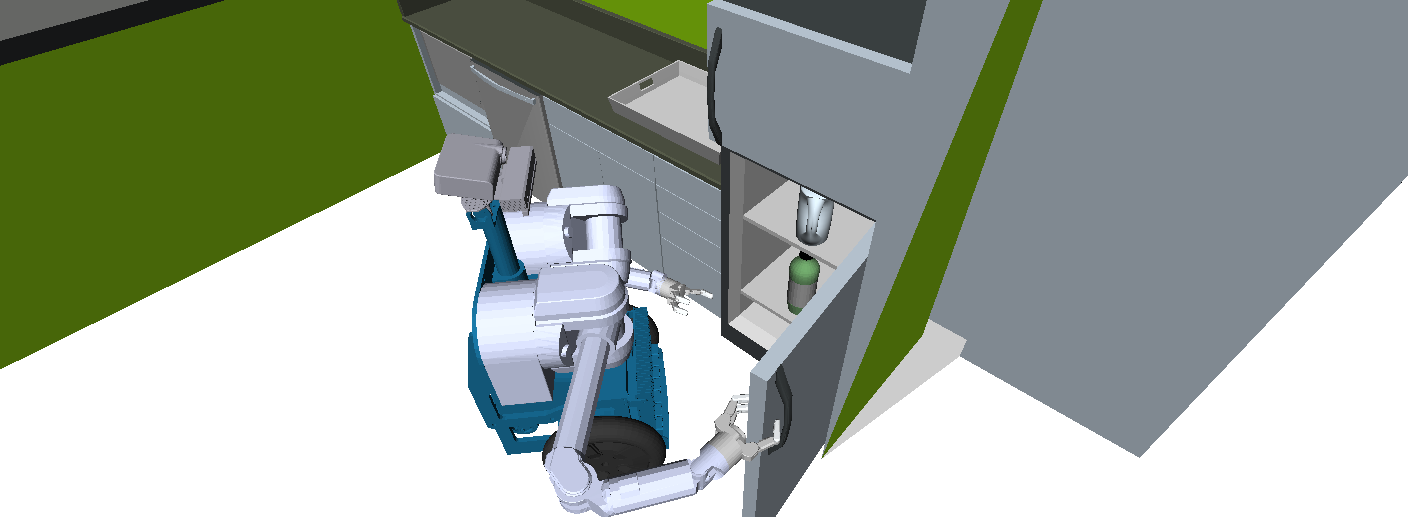
\includegraphics[width=11.5cm]{figs/herb-fridge-a.png}}%
      \only<3>{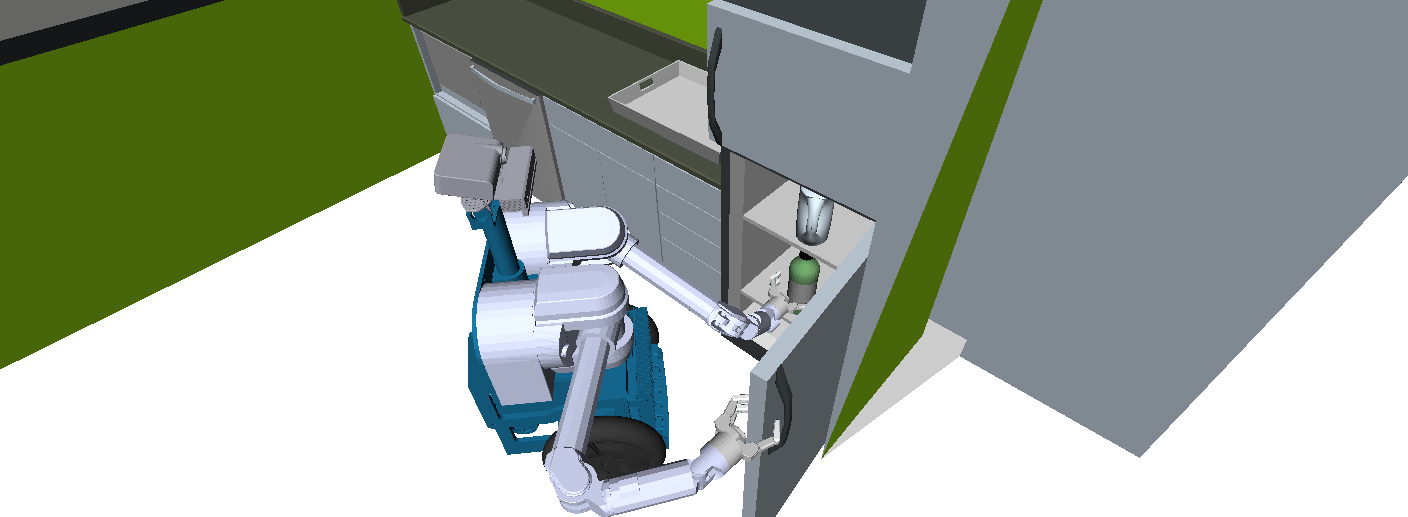
\includegraphics[width=11.5cm]{figs/herb-fridge-b.png}}%
      \only<4>{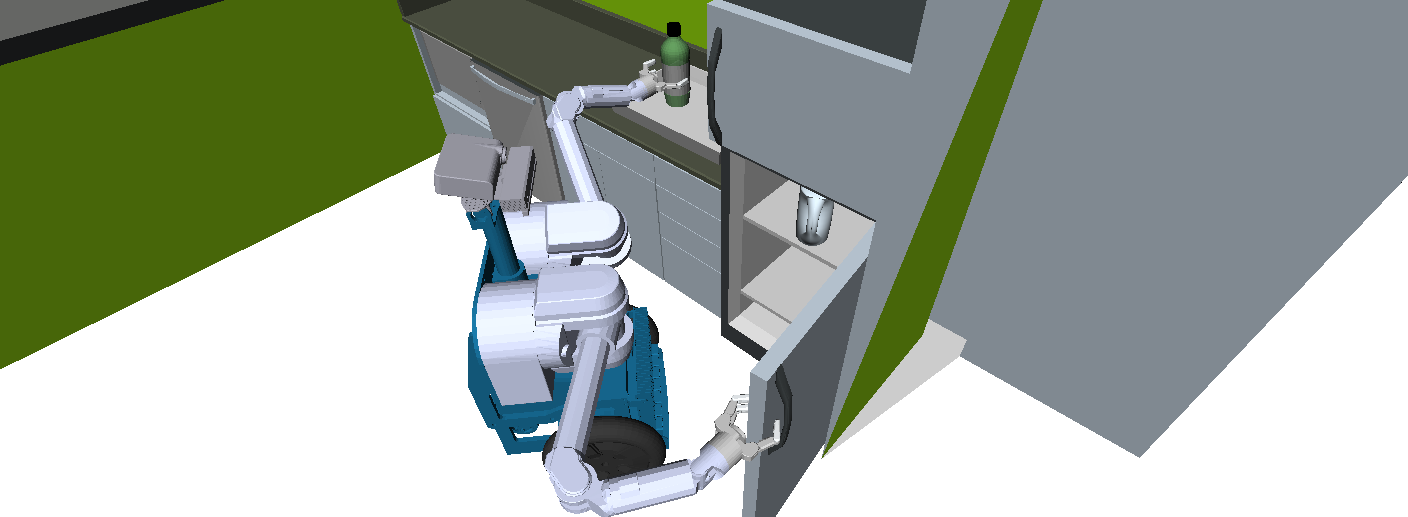
\includegraphics[width=11.5cm]{figs/herb-fridge-c.png}}%
      \only<5>{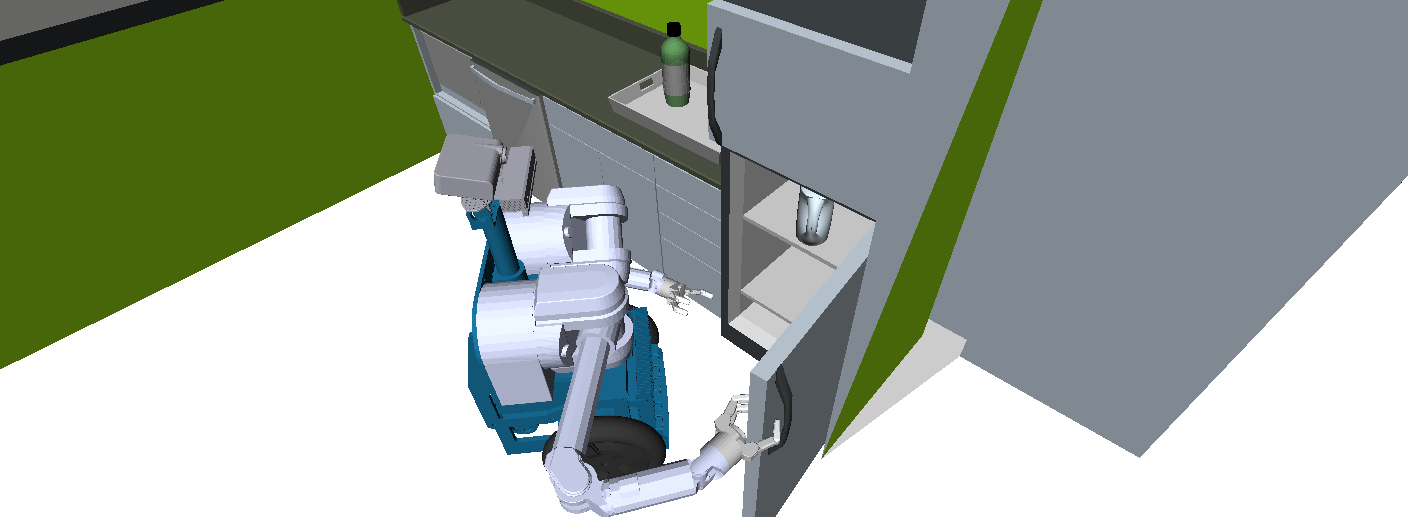
\includegraphics[width=11.5cm]{figs/herb-fridge-d.png}}%
   };

   % figure adapted from proposal doc
   \begin{scope}[font=\scriptsize,shift={(1.5,1.5)}]
      
      % root sets
      \only<3->{
         \node[draw,black,rounded corners,minimum height=1.5cm,minimum width=1cm]
            (Xgrasp) at (3,0) {};
         \node[above=0cm of Xgrasp] {Grasp};
      }
      \only<4->{
         \node[draw,black,rounded corners,minimum height=1.5cm,minimum width=1cm]
            (Xdrop) at (6,0) {};
         \node[above=0cm of Xdrop] {Place};
      }
      
      % nodes
      \only<2->
      {
         \node[circle,fill=black,inner sep=2] (xstart) at (0,0) {};
         \node[above=0.1cm of xstart] {$q_{\mbox{\scriptsize start}}$};
      }
      %\node[circle,fill=black,inner sep=2] (xg1) at (2.8,0.5) {};
      %\node[circle,fill=black,inner sep=2] (xg2) at (3.1,0.1) {};
      \only<3->{
         \node[circle,fill=black,inner sep=2] (xg3) at (2.9,-0.5) {};
      }
      \only<4->{
         \node[circle,fill=black,inner sep=2] (xd1) at (5.9,0.3) {};
      }
      %\node[circle,fill=black,inner sep=2] (xd2) at (6.0,-0.4) {};
      \only<5->
      {
         \node[circle,fill=black,inner sep=2] (xend) at (9,0) {};
         \node[above=0.1cm of xend] {$q_{\mbox{\scriptsize end}}$};
      }
      
      \only<3->{
         % in S1
         %\draw[line width=1.5mm,white]
         %   (xstart) .. controls (1,0.2) and (1.4,0.9) .. (xg1);
         %\draw[line width=1.5mm,white]
         %   (xstart) .. controls (1.5,0.2) .. (xg2);
         \draw[line width=1.5mm,white]
            (xstart) .. controls (1.8,-0.6) and (1.6,-0.8) .. (xg3);
         %\draw
         %   (xstart) .. controls (1,0.2) and (1.4,0.9) .. (xg1);
         %\draw
         %   (xstart) .. controls (1.5,0.2) .. (xg2);
         \draw
            (xstart) .. controls (1.8,-0.6) and (1.6,-0.8) .. (xg3);
      }
      
      \only<4->{
         % in s2
         %\draw[line width=1.5mm,white]
         %   (xg1) -- (4.7,0.6);
         %\draw[line width=1.5mm,white]
         %   (xg2) .. controls (4.5,1) and (3.5,-1.2) .. (4.5,-0.4)
         %         .. controls (5.5,0.5) and (5.0,-1.3) .. (xd2);
         %\draw
         %   (xg1) -- (4.7,0.6);
         %\draw
         %   (xg2) .. controls (4.5,1) and (3.5,-1.2) .. (4.5,-0.4)
         %         .. controls (5.5,0.5) and (5.0,-1.3) .. (xd2);
         \draw[line width=1.5mm,white]
            (xg3) .. controls (4.3, 0.2) and (4.5,-0.2) .. (xd1);
         \draw
            (xg3) .. controls (4.3, 0.2) and (4.5,-0.2) .. (xd1);
      }
      
      \only<5->{
         % in s3
         \draw[line width=1.5mm,white]
            (xd1) .. controls (8,0.3) and (8,0.1) .. (xend);
         \draw
            (xd1) .. controls (8,0.3) and (8,0.1) .. (xend);
      }
      
      \only<3->{
         \node[fill,black,rounded corners,minimum height=1.5cm,minimum width=1cm,
            opacity=0.1] at (3,0) {};
      }
      \only<4->{
         \node[fill,black,rounded corners,minimum height=1.5cm,minimum width=1cm,
            opacity=0.1] at (6,0) {};
      }
      
      %\draw [decorate,decoration={brace,mirror,amplitude=5pt}]
      %(0.0,-0.9) -- (2.9,-0.9) node [black,midway,yshift=-0.4cm,align=center]
      %   {bottle in fridge};

      %\draw [decorate,decoration={brace,mirror,amplitude=5pt}]
      %(3.1,-0.9) -- (5.9,-0.9) node [black,midway,yshift=-0.4cm,align=center]
      %   {bottle in hand};

      %\draw [decorate,decoration={brace,mirror,amplitude=5pt}]
      %(6.1,-0.9) -- (9.0,-0.9) node [black,midway,yshift=-0.4cm,align=center]
      %   {bottle on tray};
   \end{scope}

   %\node[inner sep=0pt] at (6,2.25) {
   %   \includegraphics{build/intro-subprob-cspace}
   %};
   
   %In order to describe why it's so slow,
   %I need to talk a bit about the problem's structure
   %and current approaches to handling it.
   %
   %I will be using this HERB example (removing items from a fridge)
   %throughout the talk.
   %
   %Below, show a 2D diagram of three steps of this plan,
   %which I then reference in the next three challenge slides.
   
   \end{tikzpicture}
\end{frame}


\begin{frame}
   \frametitle{Challenge 1: Motion Planning is Expensive}
   \begin{tikzpicture}[font=\small]
      \draw[step=1,black!15,very thin,opacity=\gridopacity] (0,0) grid (12,8);

   \node[inner sep=0pt] at (3,5.3) {%
      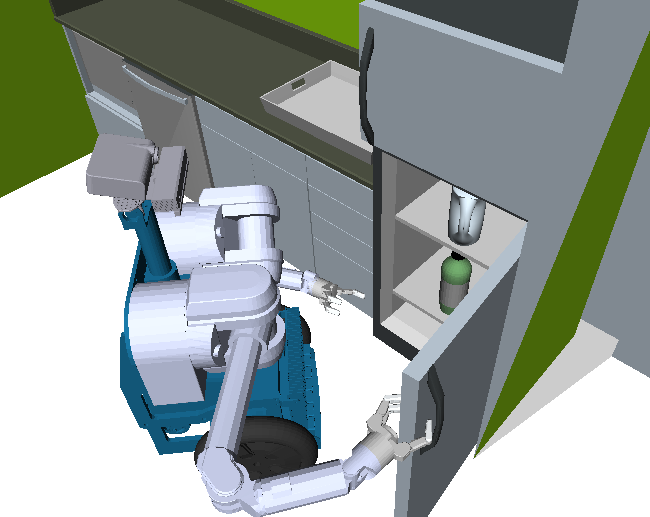
\includegraphics[width=5.75cm]{figs/herb-fridge-a-skinny.png}
   };

   \only<3->{
      \node[fill=black!10,rounded corners,font=\small,anchor=north] at (9,7.5)
         {\begin{minipage}{5.5cm}

            Configuration space $\mathcal{C}$ is:
            \only<4->{
               \begin{itemize}[leftmargin=*,itemsep=0pt,topsep=2pt]
               \item continuous, high dimensional
               \only<5->{\\$\rightarrow$ many candidate paths}
               \end{itemize}
            }
         
            \only<7->{
               \medskip
               Valid subset $\mathcal{C}_{\ms{free}}$ is:
            }
            \only<8->{
               \begin{itemize}[leftmargin=*,itemsep=0pt,topsep=2pt]
               \item induced by complex geometry
               \only<9->{\\$\rightarrow$ expensive to validate paths}
               \end{itemize}
            }

            \only<12->{
               \medskip
               Choices can render subsequent steps:
            }
            \only<13->{
               \begin{itemize}[leftmargin=*,itemsep=0pt,topsep=2pt]
               \item {\bf{impossible}} \only<15->{or {\bf{difficult}}}
               \only<18->{\\$\rightarrow$ long planning horizons}
               \end{itemize}
            }
            
            %\only<11->{
            %   \begin{center}
            %      {\bf Planning is expensive!}
            %   \end{center}
            %}
            
         \end{minipage}};
   }
   
   %\only<11->{
   %   \node[fill=blue!20,rounded corners,font=\small,anchor=north] at (9,3)
   %      {\begin{minipage}{5.5cm}
   %         \begin{center}
   %         For manipulation tasks,\\
   %         planning effort $\approx$ execution effort
   %         \end{center}
   %      \end{minipage}};
   %}
   %
   %\only<12->{
   %   \node[fill=blue!20,rounded corners,font=\small,anchor=north] at (9,1.75)
   %      {\begin{minipage}{5.5cm}
   %         \begin{center}
   %         Robot's effort spent planning
   %         detracts directly from available
   %         task resource budget.
   %         \end{center}
   %      \end{minipage}};
   %}

   % figure adapted from proposal doc
   \only<1-18>{
   \begin{scope}[font=\scriptsize,shift={(1.5,1.5)}]
      
      % root sets
      \node[draw,black,rounded corners,minimum height=1.5cm,minimum width=1cm]
         (Xgrasp) at (3,0) {};
      \node[above=0cm of Xgrasp] {Grasp};
      \only<11->{
         \node[draw,black,rounded corners,minimum height=1.5cm,minimum width=1cm]
            (Xdrop) at (6,0) {};
         \node[above=0cm of Xdrop] {Place};
      }      
      
      % cspace sets (lines only)
      \only<2-9>{
         \node[draw,black,rounded corners,minimum height=1.8cm,minimum width=1.8cm,dashed]
            (S1) at (1.5,0) {};
         \node[above left=-0.7cm of S1] {$\mathcal{C}$};
      }
      
      % nodes
      \node[circle,fill=black,inner sep=2] (xstart) at (0,0) {};
      \node[above=0.1cm of xstart] {$q_{\mbox{\scriptsize start}}$};
      \only<1-9>{
         \node[circle,fill=black,inner sep=2] (xg3) at (2.9,-0.5) {};
      }
      
      % in S1
      \only<1-9>{
      \draw[line width=1.5mm,white]
         (xstart) .. controls (1.8,-0.6) and (1.6,-0.8) .. (xg3);
      }
      
      % draw s1 cfree
      \only<6-9>{
         \begin{scope}[even odd rule]
            \clip[rounded corners] (0.61,-0.89) rectangle (2.39,0.89);
            \clip[rotate around={10:(1.1,0.5)}] (-3,-3) rectangle (3,3)
                     (0.6,-0.0) rectangle (1.6,1.0);
            \fill[blue!15,rotate around={-15:(1.5,-0.5)}] (1.5,-0.5) ellipse (1.4cm and 0.5cm);
            \fill[blue!15,rotate around={-25:(1.5, 1.0)}] (1.5, 1.0) ellipse (1.4cm and 0.5cm);
         \end{scope}
         \node[draw,inner sep=0,fill=blue!20,minimum width=0.5cm,minimum height=0.2cm]
            (Cfreebox1) at (1.2, -1.2) {};
         \node[right=0cm of Cfreebox1] {: $\mathcal{C}_{\mbox{\tiny free}}$}; 
      }

      \only<1-9>{
      \draw
         (xstart) .. controls (1.8,-0.6) and (1.6,-0.8) .. (xg3);
      }
      
      %\draw [decorate,decoration={brace,mirror,amplitude=5pt}]
      %(0.0,-0.9) -- (2.9,-0.9) node [black,midway,yshift=-0.4cm,align=center]
      %   {bottle in fridge};

      %\draw [decorate,decoration={brace,mirror,amplitude=5pt}]
      %(3.1,-0.9) -- (5.9,-0.9) node [black,midway,yshift=-0.4cm,align=center]
      %   {bottle in hand};

      %\draw [decorate,decoration={brace,mirror,amplitude=5pt}]
      %(6.1,-0.9) -- (9.0,-0.9) node [black,midway,yshift=-0.4cm,align=center]
      %   {bottle on tray};






      \only<11->{
         % grasp choices
         \node[circle,fill=black,inner sep=2] (xg1) at (2.8,0.5) {};
         \node[circle,fill=black,inner sep=2] (xg2) at (3.1,0.1) {};
         \node[circle,fill=black,inner sep=2] (xg3) at (2.9,-0.5) {};
         % place choices
         \node[circle,fill=black,inner sep=2] (xd1) at (5.9,0.3) {};
         \node[circle,fill=black,inner sep=2] (xd2) at (6.0,-0.4) {};
         % xend 
         \node[circle,fill=black,inner sep=2] (xend) at (9,0) {};
         \node[above=0.1cm of xend] {$q_{\mbox{\scriptsize end}}$};
      }
      
      %\only<2->{
      %   
      %}
      
      % in S1
      \only<12->{
         \draw[line width=1.5mm,white]
            (xstart) .. controls (1,0.2) and (1.4,0.9) .. (xg1);
      }
      \only<14->{
         \draw[line width=1.5mm,white]
            (xstart) .. controls (1.5,0.2) .. (xg2);
      }
      \only<16->{
         \draw[line width=1.5mm,white]
            (xstart) .. controls (1.8,-0.6) and (1.6,-0.8) .. (xg3);
      }
      \only<12->{
         \draw
            (xstart) .. controls (1,0.2) and (1.4,0.9) .. (xg1);
      }
      \only<14->{
         \draw
            (xstart) .. controls (1.5,0.2) .. (xg2);
      }
      \only<16->{
         \draw
            (xstart) .. controls (1.8,-0.6) and (1.6,-0.8) .. (xg3);
      }
      
      % in s2
      \only<13->{
         \draw[line width=1.5mm,white]
            (xg1) -- (4.7,0.6);
         \draw
            (xg1) -- (4.7,0.6);
      }
      \only<15->{
         \draw[line width=1.5mm,white]
            (xg2) .. controls (4.5,1) and (3.5,-1.2) .. (4.5,-0.4)
                  .. controls (5.5,0.5) and (5.0,-1.3) .. (xd2);
         \draw
            (xg2) .. controls (4.5,1) and (3.5,-1.2) .. (4.5,-0.4)
                  .. controls (5.5,0.5) and (5.0,-1.3) .. (xd2);
      }
      
      \only<17->{
         \draw[line width=1.5mm,white]
            (xg3) .. controls (4.3, 0.2) and (4.5,-0.2) .. (xd1);
         \draw
            (xg3) .. controls (4.3, 0.2) and (4.5,-0.2) .. (xd1);
      }
      
      \only<18->{
         % in s3
         \draw[line width=1.5mm,white]
            (xd1) .. controls (8,0.3) and (8,0.1) .. (xend);
         \draw
            (xd1) .. controls (8,0.3) and (8,0.1) .. (xend);
      }

      \node[fill,black,rounded corners,minimum height=1.5cm,minimum width=1cm,
         opacity=0.1] at (3,0) {};
      \only<11->{
         \node[fill,black,rounded corners,minimum height=1.5cm,minimum width=1cm,
            opacity=0.1] at (6,0) {};
      }
      
   \end{scope}
   }

   \only<19->{
      \node[fill=blue!15,rounded corners,font=\small] at (6,1.75)
      {\begin{minipage}{11cm}\large

         \emph{Q1: {\bf \emph{How can we optimize}}
         paths for motion planning problems
         %in manipulation tasks
         in the face of expensive validity checking?}

      \end{minipage}};
   }

   \end{tikzpicture}
\end{frame}






\begin{frame}
   \frametitle{Challenge 2: Capturing the Plan/Execute Tradeoff}
   \begin{tikzpicture}[font=\small]
      \draw[step=1,black!15,very thin,opacity=\gridopacity] (0,0) grid (12,8);

   \node[inner sep=0pt] at (3,5.3) {%
      \only<1-4>{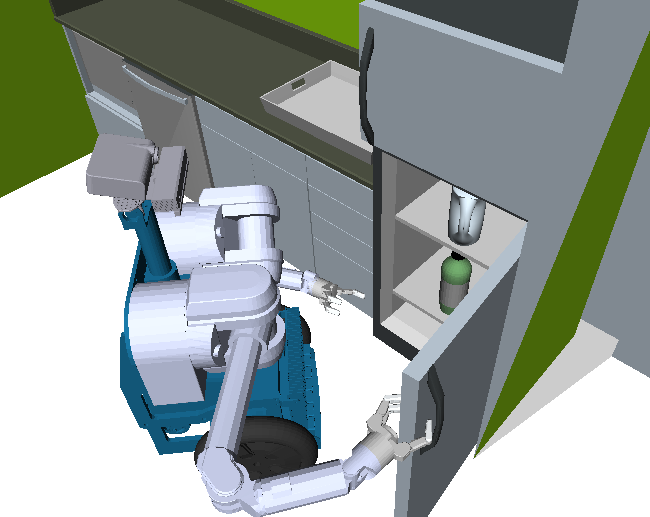
\includegraphics[width=5.75cm]{figs/herb-fridge-a-skinny.png}}%
      \only<5>{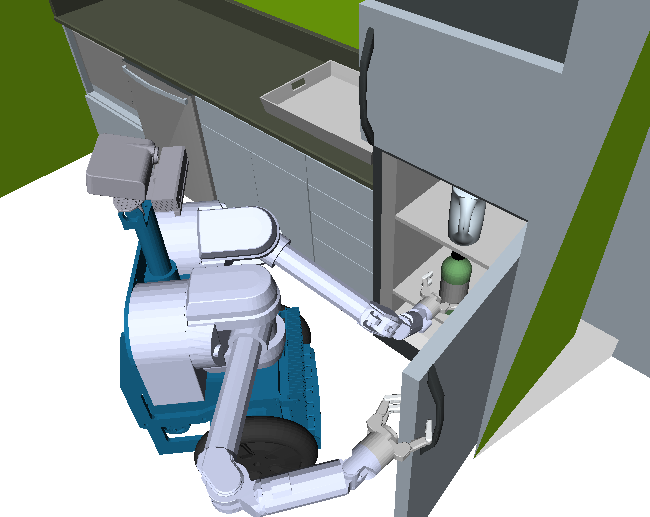
\includegraphics[width=5.75cm]{figs/herb-fridge-b-skinny.png}}%
      \only<6->{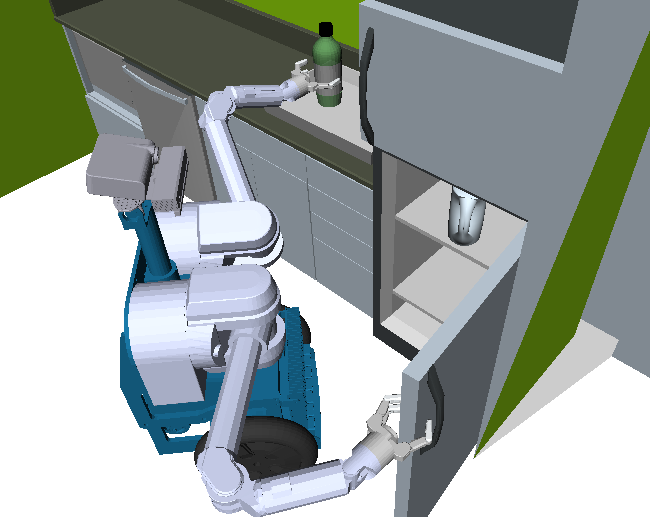
\includegraphics[width=5.75cm]{figs/herb-fridge-c-skinny.png}}%
   };

   \only<2->{
   \node[fill=black!10,rounded corners,font=\small,anchor=north] at (9,7.75)
   {\begin{minipage}{5.5cm}

      There is an {\bf explicit effort tradeoff} between
      \emph{planning motion} and \emph{executing it}.
      
      \only<3->{
      \medskip
      Existing methods require parameters
      that are often difficult to tune:
      \begin{itemize}[leftmargin=*,itemsep=0pt,topsep=2pt]
      \item planning/shortcutting budgets
      \item inflation factors
      \end{itemize}
      }

      \only<4->{
      \medskip
      Anytime planners require termination
      and may not achieve the best tradeoff.
      }

      \only<8->{
      \medskip
      Caching for fast planning is difficult
      since each step induces a distinct $\mathcal{C}_{\ms{free}}$.
      }
      
   \end{minipage}};
   }

   \only<1-8>{
   % figure adapted from proposal doc
   \begin{scope}[font=\scriptsize,shift={(1.5,1.5)}]
      
      % root sets
      \node[draw,black,rounded corners,minimum height=1.5cm,minimum width=1cm]
         (Xgrasp) at (3,0) {};
      \node[above=0cm of Xgrasp] {Grasp};
      
      \only<6->{
         \node[draw,black,rounded corners,minimum height=1.5cm,minimum width=1cm]
            (Xdrop) at (6,0) {};
         \node[above=0cm of Xdrop] {Place};
      }
      
      % cspace sets
      \only<5->{
         \node[draw,black,rounded corners,minimum height=1.8cm,minimum width=1.8cm,dashed]
            (S1) at (1.5,0) {};
         \node[above left=-0.7cm of S1] {$\mathcal{C}$};
      }
      
      \only<7->{
         \node[draw,black,rounded corners,minimum height=1.8cm,minimum width=1.8cm,dashed]
            (S1) at (4.5,0) {};
         \node[above left=-0.7cm of S1] {$\mathcal{C}$};
      }
      
      % nodes
      \node[circle,fill=black,inner sep=2] (xstart) at (0,0) {};
      \node[above=0.1cm of xstart] {$q_{\mbox{\scriptsize start}}$};
      \node[circle,fill=black,inner sep=2] (xg3) at (2.9,-0.5) {};
      
      % in S1
      \draw[line width=1.5mm,white]
         (xstart) .. controls (1.8,-0.6) and (1.6,-0.8) .. (xg3);
      % draw s1 cfree
      \only<5->{
         \begin{scope}[even odd rule]
            \clip[rounded corners] (0.61,-0.89) rectangle (2.39,0.89);
            \clip[rotate around={10:(1.1,0.5)}] (-3,-3) rectangle (3,3)
                     (0.6,-0.0) rectangle (1.6,1.0);
            \fill[blue!15,rotate around={-15:(1.5,-0.5)}] (1.5,-0.5) ellipse (1.4cm and 0.5cm);
            \fill[blue!15,rotate around={-25:(1.5, 1.0)}] (1.5, 1.0) ellipse (1.4cm and 0.5cm);
         \end{scope}
         \node[draw,inner sep=0,fill=blue!20,minimum width=0.5cm,minimum height=0.2cm]
               (Cfreebox1) at (1.2, -1.2) {};
            \node[right=0cm of Cfreebox1] {: $\mathcal{C}_{\mbox{\tiny free1}}$};
      }
      \draw
         (xstart) .. controls (1.8,-0.6) and (1.6,-0.8) .. (xg3);
      
      % in s2
      \only<6->{
         \node[circle,fill=black,inner sep=2] (xd1) at (5.9,0.3) {};
         \draw[line width=1.5mm,white]
            (xg3) .. controls (4.3, 0.2) and (4.5,-0.2) .. (xd1);
         \only<7->{
            % draw s2 cfree
            \begin{scope}[even odd rule]
               \clip[rounded corners] (3.61,-0.89) rectangle (5.39,0.89);
               \clip[rotate around={10:(4.1,0.5)}] (0,-3) rectangle (6,3)
                     (3.6,-0.0) rectangle (4.6,1.0);
               \fill[red!15,rotate around={15:(4.5,-0.2)}] (4.5,-0.2) ellipse (1.4cm and 0.5cm);
            \end{scope}
            \node[draw,inner sep=0,fill=red!20,minimum width=0.5cm,minimum height=0.2cm]
               (Cfreebox1) at (4.2, -1.2) {};
            \node[right=0cm of Cfreebox1] {: $\mathcal{C}_{\mbox{\tiny free2}}$};
         }
         \draw
            (xg3) .. controls (4.3, 0.2) and (4.5,-0.2) .. (xd1);
      }
      
      \node[fill,black,rounded corners,minimum height=1.5cm,minimum width=1cm,
         opacity=0.1] at (3,0) {};
      \only<6->{
         \node[fill,black,rounded corners,minimum height=1.5cm,minimum width=1cm,
            opacity=0.1] at (6,0) {};
      }
      
      %\draw [decorate,decoration={brace,mirror,amplitude=5pt}]
      %(0.0,-0.9) -- (2.9,-0.9) node [black,midway,yshift=-0.4cm,align=center]
      %   {bottle in fridge};

      %\draw [decorate,decoration={brace,mirror,amplitude=5pt}]
      %(3.1,-0.9) -- (5.9,-0.9) node [black,midway,yshift=-0.4cm,align=center]
      %   {bottle in hand};

      %\draw [decorate,decoration={brace,mirror,amplitude=5pt}]
      %(6.1,-0.9) -- (9.0,-0.9) node [black,midway,yshift=-0.4cm,align=center]
      %   {bottle on tray};

   \end{scope}
   }

   \only<9->{
      \node[fill=blue!15,rounded corners,font=\small] at (6,1.75)
      {\begin{minipage}{11cm}\large

         \emph{Q2: {\bf \emph{What should we optimize}}
         to effectively trade off between planning and execution cost
         over a manipulation task?}

      \end{minipage}};
   }

   \end{tikzpicture}
\end{frame}

